\chapter{Quality of Service}\label{Chapter:QoS}
\section{The DDS QoS Model} \label{Section:DDS:QoS} \index{QoS Model}
\begin{figure}[t]
	\centering
	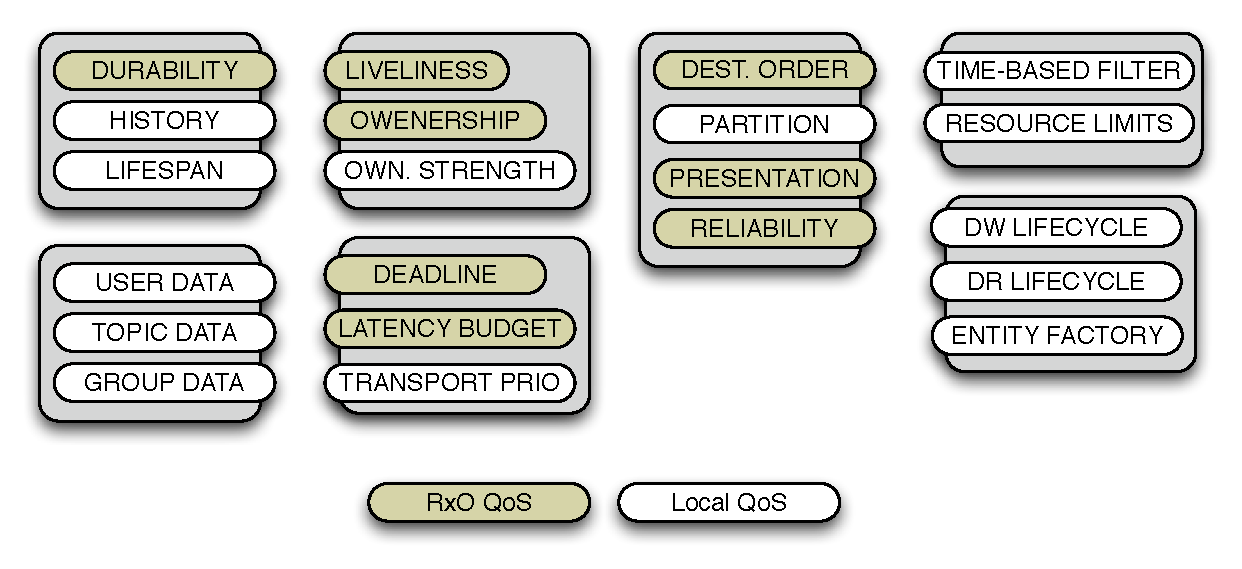
\includegraphics[scale=0.6]{figs/QoS-Map.eps}
	\caption{DDS QoS Policies.}
	\label{Figure:DDS:QoSMap}
\end{figure}
%%%
\ac{DDS} provides applications policies to control a wide set
of non-functional properties, such as data availability, data
delivery, data timeliness and resource usage -- Figure~\ref{Figure:DDS:QoSMap} shows
the full list of available QoS.  
The semantics and the behaviour of \ac{DDS} entities, such as a topic, data
reader, and data writer, can be controlled through available \ac{QoS}
policies.  The policies that control and end-to-end property are
considered as part of the subscription matching. 
%%%
\begin{figure}[t]
	\centering
	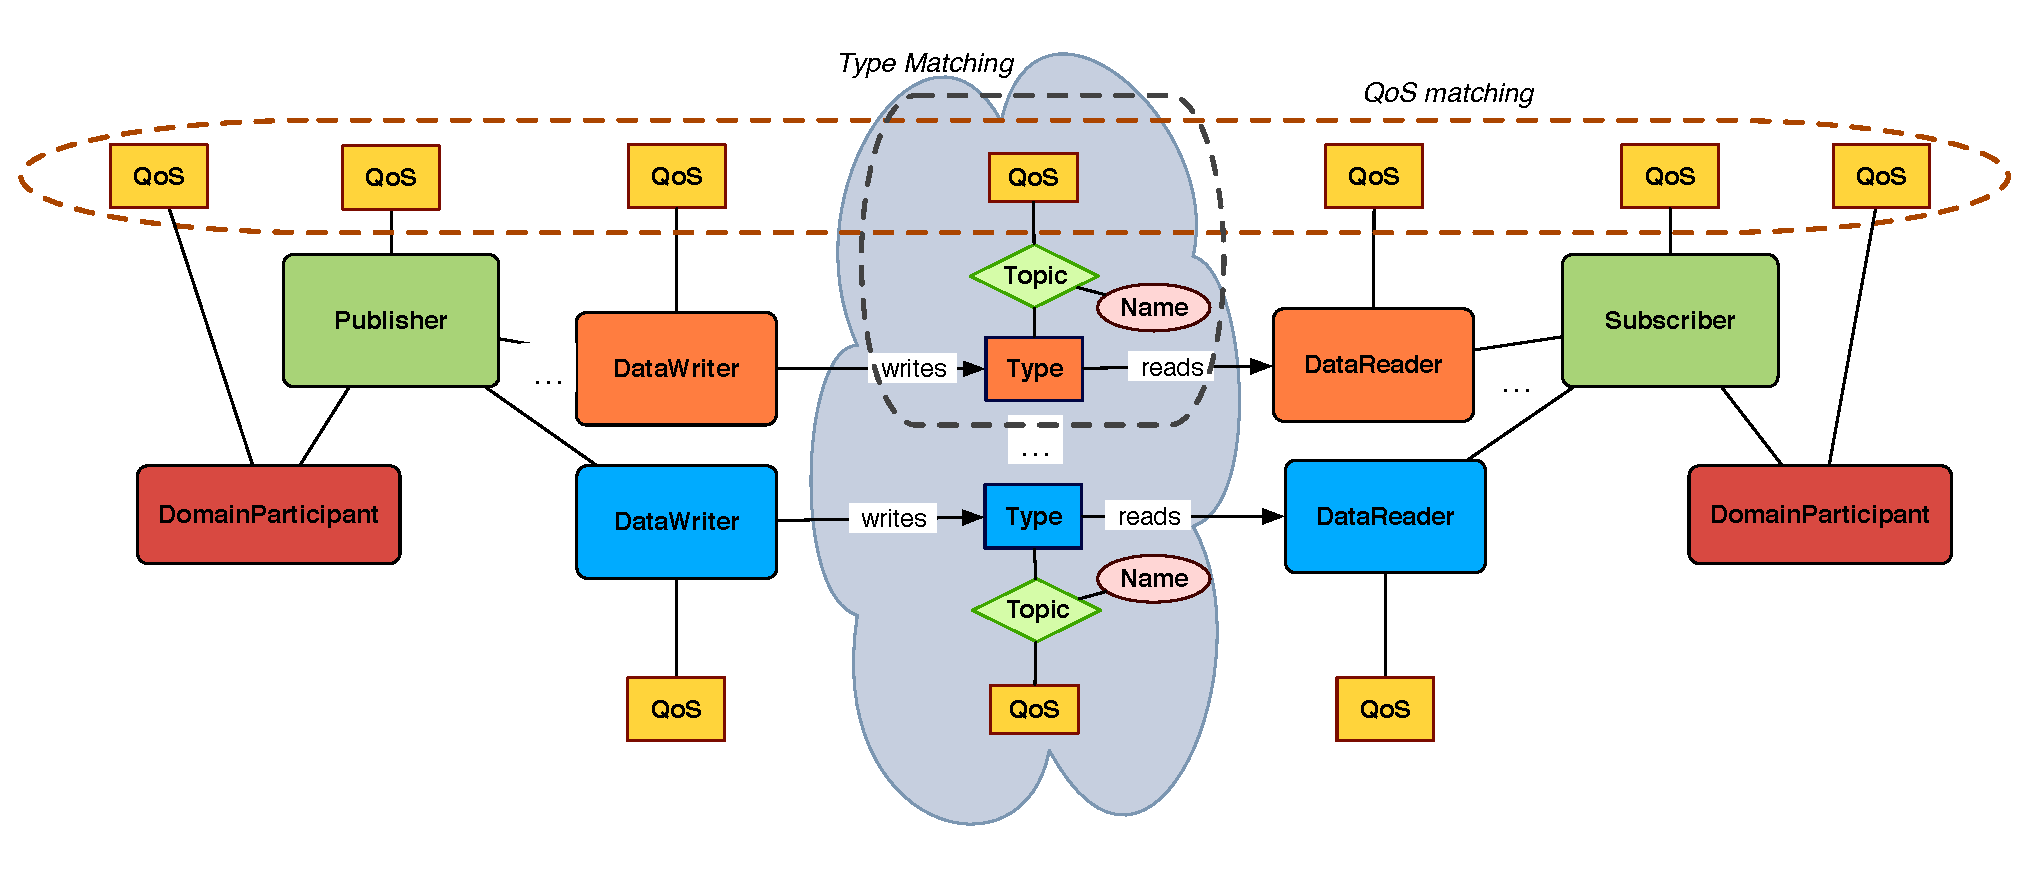
\includegraphics[scale=0.4]{figs/RxO.eps}
	\caption{DDS Request vs. Offered QoS Model.}
	\label{Figure:DDS:RxO}
\end{figure}
%%%
\ac{DDS} uses a request vs. offered QoS matching approach, as
shown in Figure~\ref{Figure:DDS:RxO} in which a
data reader matches a data writer if and only if the QoS it is
requesting for the given topic does not exceed (e.g., is no more
stringent) than the QoS with which the data is produced by the data
writer.  

\ac{DDS} subscriptions are matched against the topic type and
name, as well as against the \ac{QoS} being offered\-/requested by
data writers and readers.  This DDS matching mechanism ensures that
(1) types are preserved end-to-end due to the topic type matching and
(2) end-to-end \ac{QoS} invariants are also preserved.

The reminder of this section describes the most important \ac{QoS}
policies in \ac{DDS}.

\subsection{Data availability} \index{Data Availability QoS}
DDS provides the following QoS policies that control the availability
of data to domain participants:
\begin{itemize}

	\item The \texttt{DURABILITY} \ac{QoS} policy controls the
          lifetime of the data written to the global data space in a
          \ac{DDS} domain.  Supported durability levels include (1)
          \texttt{VOLATILE}, which specifies that once data is
          published it is not maintained by \ac{DDS} for delivery to
          late joining applications, (2) \texttt{TRANSIENT\_LOCAL},
          which specifies that publishers store data locally so that
          late joining subscribers get the last published item if a
          publisher is still alive, (3) \texttt{TRANSIENT}, which
          ensures that the \ac{GDS} maintains the information outside
          the local scope of any publishers for use by late joining
          subscribers, and (4) \texttt{PERSISTENT}, which ensures that
          the \ac{GDS} stores the information persistently so to make
          it available to late joiners even after the shutdown and
          restart of the whole system.  Durability is achieved by
          relying on a durability service whose properties are
          configured by means of the \texttt{DURABILITY\_SERVICE}
          \ac{QoS} of non-volatile topics.

	\item The \texttt{LIFESPAN} \ac{QoS} policy controls the
          interval of time during which a data sample is valid. The
          default value is infinite, with alternative values being the
          time-span for which the data can be considered valid.

	\item The \texttt{HISTORY} \ac{QoS} policy controls the number
          of data samples (i.e., subsequent writes of the same topic)
          that must be stored for readers or writers. Possible values
          are the last sample, the last $n$ samples, or all samples.
\end{itemize}
These \ac{DDS} data availability \ac{QoS} policies decouple
applications in time and space.  They also enable these applications
to cooperate in highly dynamic environments characterized by
continuous joining and leaving of publisher\-/subscribers.  Such
properties are particularly relevant in \ac{SoS} since they increase
the decoupling of the component parts.

\subsection{Data delivery} \index{Data Delivery QoS}
DDS provides the following QoS policies that control how data is
delivered and how publishers can claim exclusive rights on data
updates:
%%%
\begin{itemize}
	\item The \texttt{PRESENTATION} QoS policy gives control on
          how changes to the information model are presented to
          subscribers. This \ac{QoS} gives control on the ordering as
          well as the coherency of data updates.  The scope at which
          it is applied is defined by the access scope, which can be
          one of \texttt{INSTANCE}, \texttt{TOPIC}, or \texttt{GROUP}
          level.

	\item The \texttt{RELIABILITY} QoS policy controls the level
          of reliability associated with data diffusion. Possible
          choices are \texttt{RELIABLE} and \texttt{BEST\_EFFORT}
          distribution.

	\item The \texttt{PARTITION} \ac{QoS} policy gives control
          over the association between \ac{DDS} partitions
          (represented by a string name) and a specific instance of a
          publisher/subscriber.  This association provides \ac{DDS}
          implementations with an abstraction that allow to segregate
          traffic generated by different partitions, thereby improving
          overall system scalability and performance.
	
 	\item The \texttt{DESTINATION\_ORDER} \ac{QoS} policy controls
          the order of changes made by publishers to some instance of
          a given topic. DDS allows the ordering of different changes
          according to source or destination timestamps.

	\item The \texttt{OWNERSHIP} \ac{QoS} policy controls which
          writer ``owns'' the write-access to a topic when there are
          multiple writers and ownership is \texttt{EXCLUSIVE}. Only
          the writer with the highest \texttt{OWNERSHIP\_STRENGTH} can
          publish the data.  If the \texttt{OWNERSHIP} \ac{QoS} policy
          value is shared, multiple writers can concurrently update a
          topic. \texttt{OWNERSHIP} thus helps to manage replicated
          publishers of the same data.
	
\end{itemize}
These \ac{DDS} data delivery \ac{QoS} policies control the reliability
and availability of data, thereby allowing the delivery of the right
data to the right place at the right time.  More elaborate ways of
selecting the right data are offered by the \ac{DDS} content-awareness
profile, which allows applications to select information of interest
based upon their content.  These \ac{QoS} policies are particularly
useful in \ac{SoS} since they can be used to finely tune how---and to
whom---data is delivered, thus limiting not only the amount of
resources used, but also minimizing the level of interference by
independent data streams.

\subsection{Data timeliness} \index{Data Timeliness QoS}
DDS provides the following \ac{QoS} policies to control the timeliness
properties of distributed data:
%%%
\begin{itemize}

	\item The \texttt{DEADLINE} \ac{QoS} policy allows
          applications to define the maximum inter-arrival time for
          data. \ac{DDS} can be configured to automatically notify
          applications when deadlines are missed.

	\item The \texttt{LATENCY\_BUDGET} QoS policy provides a means
          for applications to inform \ac{DDS} of the urgency
          associated with transmitted data.  The latency budget
          specifies the time period within which \ac{DDS} must
          distribute the information. This time period starts from the
          moment the data is written by a publisher until it is
          available in the subscriber’s data-cache ready for use by
          reader(s).

	\item The \texttt{TRANSPORT\_PRIORITY} QoS policy allows
          applications to control the importance associated with a
          topic or with a topic instance, thus allowing a DDS
          implementation to prioritize more important data relative to
          less important data. These QoS policies help ensure that
          mission-critical information needed to reconstruct the
          shared operational picture is delivered in a timely manner.
\end{itemize}
These \ac{DDS} data timeliness \ac{QoS} policies provide control over
the temporal properties of data.  Such properties are particularly
relevant in \ac{SoS} since they can be used to define and control the
temporal aspects of various subsystem data exchanges, while ensuring
that bandwidth is exploited optimally.

\subsection{Resources} \index{Resource Control QoS}
\ac{DDS} defines the following \ac{QoS} policies to control the
network and computing resources that are essential to meet data
dissemination requirements:
\begin{itemize}

	\item The \texttt{TIME\_BASED\_FILTER} \ac{QoS} policy allows
          applications to specify the minimum inter-arrival time
          between data samples, thereby expressing their capability to
          consume information at a maximum rate. Samples that are
          produced at a faster pace are not delivered. This policy
          helps a \ac{DDS} implementation optimize network bandwidth,
          memory, and processing power for subscribers that are
          connected over limited bandwidth networks or which have
          limited computing capabilities.

	\item The \texttt{RESOURCE\_LIMITS} \ac{QoS} policy allows
          applications to control the maximum available storage to
          hold topic instances and related number of historical
          samples \ac{DDS}’s \ac{QoS} policies support the various
          elements and operating scenarios that constitute net-centric
          mission-critical information management. By controlling
          these QoS policies it is possible to scale \ac{DDS} from
          low-end embedded systems connected with narrow and noisy
          radio links, to high-end servers connected to high-speed
          fiber-optic networks.
\end{itemize}
These \ac{DDS} resource \ac{QoS} policies provide control over the
local and end-to-end resources, such as memory and network bandwidth.
Such properties are particularly relevant in \ac{SoS} since they are
characterized by largely heterogeneous subsystems, devices, and
network connections that often require down-sampling, as well as
overall controlled limit on the amount of resources used.

\subsection{Configuration} \index{Configuration QoS}
The \ac{QoS} policies described above, provide control over the most
important aspects of data delivery, availability, timeliness, and
resource usage.  \ac{DDS} also supports the definition and
distribution of user specified bootstrapping information via the
following QoS policies:

\begin{itemize}
%%%
	\item The \texttt{USER\_DATA} \ac{QoS} policy allows
          applications to associate a sequence of octets to domain
          participant, data readers and data writers. This data is
          then distributed by means of a built-in topic. This QoS
          policy is commonly used to distribute security credentials.

	\item The \texttt{TOPIC\_DATA} \ac{QoS} policy allows
          applications to associate a sequence of octet with a
          topic. This bootstrapping information is distributed by
          means of a built-in topic. A common use of this \ac{QoS}
          policy is to extend topics with additional information, or
          meta-information, such as IDL type-codes or XML schemas.

	\item The \texttt{GROUP\_DATA} \ac{QoS} policy allows
          applications to associate a sequence of octets with
          publishers and subscribers--this bootstrapping information
          is distributed by means built-in topics.  A typical use of
          this information is to allow additional application control
          over subscriptions matching.
\end{itemize}
These \ac{DDS} configuration \ac{QoS} policies provide useful a
mechanism for bootstrapping and configuring applications that run in
\ac{SoS}.  This mechanism is particularly relevant in \ac{SoS} since
it provides a fully distributed means of providing configuration
information.


\subsection{Setting QoS}
All the code examples you have have seen so far did rely on default \ac{QoS} 
settings, as such we did not have to be concerned with defining the desired 
\ac{QoS}. Listing~\ref{Listing:DDS:QoS} shows how you can create and set 
\ac{QoS} on \ac{DDS} entities. 


%%%
%%%
\iftoggle{cpp}{
	\lstinputlisting[
		frame=b,
		label={Listing:DDS:QoS},
		caption={Setting QoS on DDS entities.}]
		{./listing/cxx/qos-example.cpp}
}
%%%

Along with an API to explicitly create \ac{QoS}, \ac{DDS} also provides
the concept of a \texttt{QoSProvider} to make it possible to externalize the 
definition of the \ac{QoS} and make it a deployment time concern.
The listing below show how the \texttt{QoSProvider} can be used to fetch
\ac{QoS} definition from a file. 

%%%
\iftoggle{cpp}{
	\lstinputlisting[
		frame=b,
		label={Listing:DDS:QoS},
		caption={Setting QoS on DDS entities using the QoSProvider.}]
		{./listing/cxx/qos-provider.cpp}
}
%%%

\section{Summary}
In this chapter I've explained the role of \ac{QoS} in \ac{DDS} and shown how 
the various policies can be used to control the most important aspects of 
communication, data availability and resource usage. 
The code example have also illustrated that setting \ac{QoS} is pretty straightforward
and the use of the \texttt{QoSProvider} can be of great help in making the selection
of \ac{QoS} a deployment concern.
